\chapter{Model Architecture and Resource Requirements}

\section*{Why This Matters}

Model architecture decisions—dimensions, layers, parameter counts—directly determine infrastructure requirements, operational costs, and system performance. Understanding the relationship between architectural choices and resource consumption is essential for evaluating technical proposals, planning infrastructure investments, and making informed build-versus-buy decisions.

The computational characteristics of neural networks follow predictable patterns. A model's parameter count, layer structure, and dimensional choices create specific memory footprints and computational demands. These relationships aren't linear: doubling a model's dimensions typically quadruples memory requirements and increases computation eightfold. Recognizing these scaling behaviors enables accurate cost forecasting and realistic performance expectations.

This chapter establishes the technical foundation for evaluating model architectures, focusing on how architectural parameters translate to resource requirements.

\section*{Key Questions This Chapter Answers}

By the end of this chapter, you'll be able to answer:

\begin{itemize}
    \item Why does doubling model dimensions increase costs 8×, not 2×?
    \item Where do BERT's 110M parameters actually go, and why does it matter?
    \item When does the 13× memory overhead of training versus inference become critical?
    \item How do you evaluate vendor claims about "optimized architectures"?
    \item What's the difference between compute-bound and memory-bound operations?
\end{itemize}

\textbf{Note on Examples (2026 Context):} This chapter uses BERT-base as the primary teaching example due to its clear, well-documented architecture. By 2026, BERT-base has been largely replaced in production by more efficient alternatives (DistilBERT, modern compact encoders like DeBERTa-v3, and domain-specific models). However, it remains an excellent pedagogical tool—the architectural principles and scaling laws presented here apply universally to all transformer models, from compact encoders to frontier LLMs like GPT-4, Claude 3 Opus, LLaMA 3, and Mistral Large.

\section{Mathematical Foundations: What Linear Algebra Actually Is}

Before discussing computational costs and resource requirements, it's essential to understand what linear algebra operations actually do and why they're fundamental to neural networks.

\subsection{Vectors and Matrices: Representing Data and Transformations}

At its core, linear algebra provides a mathematical framework for working with collections of numbers and transforming them systematically. In deep learning, we represent data as \textbf{vectors}—ordered lists of numbers—and transformations as \textbf{matrices}—rectangular arrays of numbers.

\textbf{Example: Image as a Vector}

A 28×28 grayscale image (like MNIST handwritten digits) contains 784 pixels, each with an intensity value. We can represent this image as a vector with 784 components—a single point in 784-dimensional space. For a color image (224×224 RGB), we have 150,528 numbers (224 × 224 × 3 channels). This is why we talk about "high-dimensional data"—images naturally live in spaces with hundreds of thousands of dimensions.

\textbf{Example: Text as a Vector}

In natural language processing, words are represented as vectors called embeddings. The word "king" might be a vector with 300 or 768 components. These embeddings are learned such that semantically similar words have similar vectors. The famous example: vector("king") - vector("man") + vector("woman") ≈ vector("queen"), showing that vector arithmetic can capture semantic relationships.

\subsection{Matrix Multiplication: The Core Transformation}

A neural network layer transforms input data by multiplying it with a weight matrix. This operation projects the data into a new representational space.

\textbf{Concrete Example:}

Consider transforming a 784-dimensional input (flattened MNIST image) to a 256-dimensional hidden representation:
\begin{itemize}
    \item Input vector: 784 numbers
    \item Weight matrix: 784 × 256 = 200,704 numbers
    \item Output vector: 256 numbers
\end{itemize}

Each of the 256 output values is computed by taking a weighted sum of all 784 input values. This requires 784 multiplications and 784 additions per output, totaling 200,704 multiply-add operations for the full transformation.

\textbf{Why This Matters:} This single layer has 200,704 trainable parameters. Understanding where parameters come from (matrix dimensions) is essential for evaluating model size claims and memory requirements.

\subsection{Dot Products: Measuring Similarity}

The dot product between two vectors measures their similarity or alignment. For vectors $\mathbf{x}$ and $\mathbf{y}$ with $n$ components:

\begin{equation}
\text{dot product} = x_1 y_1 + x_2 y_2 + \cdots + x_n y_n
\end{equation}

\textbf{Geometric Interpretation:} The dot product is large when vectors point in similar directions and small (or negative) when they point in different directions. This makes it perfect for measuring similarity.

\textbf{Application in Transformers:} Attention mechanisms use dot products to determine which words in a sentence should "attend to" each other. When processing "The cat sat on the mat," the model computes dot products between word representations to determine that "cat" and "sat" are related (subject-verb relationship).

\textbf{Concrete Example:}

Query vector for "cat": [0.5, 0.8, 0.3]
Key vector for "sat": [0.6, 0.7, 0.2]
Key vector for "mat": [-0.3, 0.1, 0.9]

Dot product (cat, sat) = 0.5×0.6 + 0.8×0.7 + 0.3×0.2 = 0.92
Dot product (cat, mat) = 0.5×(-0.3) + 0.8×0.1 + 0.3×0.9 = 0.20

The higher score (0.92) indicates "cat" should attend more to "sat" than to "mat" (0.20).

\subsection{Why These Operations Scale Cubically}

Understanding computational scaling is crucial for cost estimation:

\textbf{Matrix Storage (Quadratic):} An $n \times n$ matrix contains $n^2$ numbers. Doubling $n$ quadruples storage requirements.

\textbf{Matrix Multiplication (Cubic):} Multiplying two $n \times n$ matrices requires $n^3$ operations:
\begin{itemize}
    \item Output has $n^2$ positions (quadratic)
    \item Each position requires $n$ multiply-add operations (linear)
    \item Total: $n^2 \times n = n^3$ (cubic)
\end{itemize}

\textbf{Practical Impact:} Doubling model dimensions increases:
\begin{itemize}
    \item Parameters by 4× (quadratic)
    \item Computation by 8× (cubic)
    \item Memory by 4× (quadratic)
\end{itemize}

This is why BERT-large (1024 dimensions) requires approximately 8× more computation per layer than BERT-base (768 dimensions), despite only a 33\% dimensional increase.

\section{Computational Foundations}

\subsection{Matrix Operations as Core Primitives}

With the mathematical foundation established, we can now examine how these operations translate to computational costs. Neural networks perform transformations through matrix operations—structured mathematical operations on arrays of numbers. Each layer applies a learned transformation, implemented as matrix multiplication, to its input data. The computational cost and memory requirements scale predictably with matrix dimensions.

A transformation layer with 768-dimensional input and output requires a 768×768 weight matrix containing approximately 590,000 parameters. Each forward pass performs roughly 590,000 multiply-accumulate operations. Modern GPUs execute these operations in parallel, but the total work remains proportional to matrix size.

The critical relationship: computational cost grows cubically with dimension. A 1024-dimensional layer (33\% larger) requires 1,048,576 parameters—a 78\% increase—and performs proportionally more computation. This non-linear scaling fundamentally shapes model design decisions and cost structures.

\subsection{Matrix Multiplication: Cost Scaling Intuition}

\textbf{Intuition: The Tournament Analogy}

Think of matrix multiplication like organizing a round-robin tournament. You have n teams (rows), and each team plays n opponents (columns). That's n² matches total (quadratic). But each match requires n rounds of play to determine a winner (linear per match). Total work: n² matches × n rounds = n³ operations (cubic).

When you double the number of teams (2n), you don't just double the work. Matches increase 4× (from n² to 4n²), and rounds per match double (from n to 2n). Total work increases 8× (from n³ to 8n³). This is why "slightly larger models" explode in cost—the scaling isn't linear or even quadratic, it's cubic.

Understanding why costs scale cubically (not linearly or quadratically) is essential for evaluating architectural proposals:

For an n×n matrix multiplication C = A×B:
\begin{itemize}
    \item You have n² output positions (memory: quadratic)
    \item Each output requires n multiply-accumulate operations (computation per output: linear in n)
    \item Total computation: n² × n = n³ (cubic)
\end{itemize}

\textbf{Practical intuition}:
\begin{itemize}
    \item Double the matrix size → 2² = 4× more outputs → 2× operations per output → 8× total work
    \item This is why BERT-large (33\% larger dimensions) requires $\sim$8× longer training than BERT-base
    \item A seemingly modest 50\% dimensional increase yields 3.4× more computation
\end{itemize}

This cubic relationship is the fundamental constraint on model scaling. When evaluating proposals to increase model dimensions, remember that costs scale much faster than the dimensional parameter itself.

\subsection{Dimensional Scaling and Cost Implications}

The relationship between model dimensions and computational cost follows a cubic function. Doubling the dimensional parameter increases memory requirements by a factor of four and computational operations by a factor of eight.

BERT-base, a widely-deployed language model, uses 768-dimensional representations. Each transformation layer multiplies 768×768 matrices, requiring approximately 590,000 operations per layer. BERT-large increases dimensions to 1024, requiring 1,048,576 operations per layer—nearly double the computational load.

The compounding effect: BERT-large employs 24 layers versus BERT-base's 12. The combined impact approaches a 4× increase in total computation, despite the dimensional increase appearing modest at 33\%. This multiplicative relationship between architectural parameters and resource requirements necessitates careful analysis of proposed specifications.

\begin{figure}[htbp]
\centering
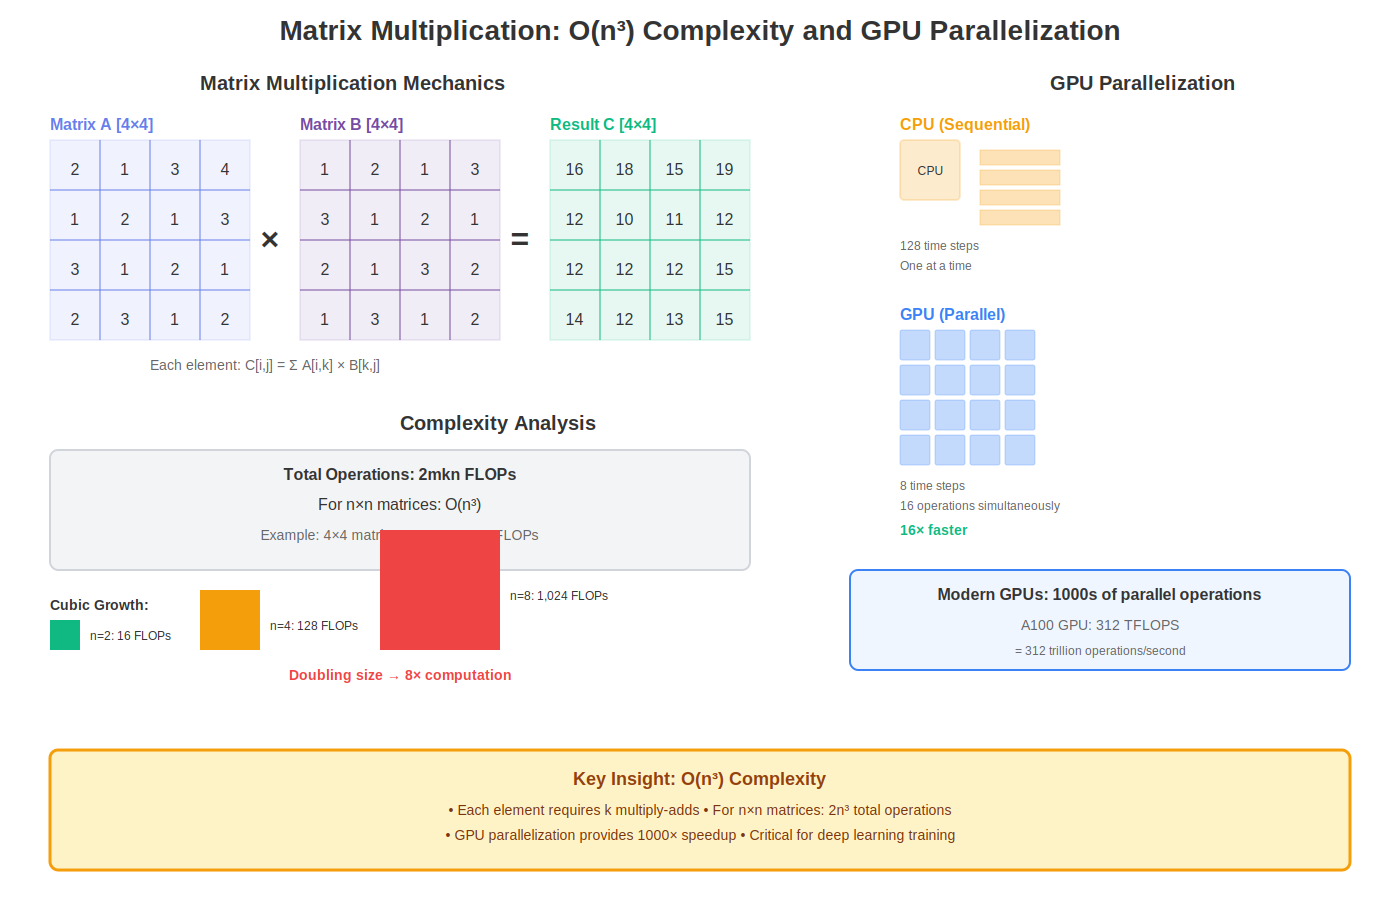
\includegraphics[width=0.95\textwidth]{chapters/diagrams/chapter01_matrix_multiplication_522a20fb.pdf}
\caption{Matrix multiplication operations showing parallel computation structure. Modern GPUs execute thousands of operations simultaneously, but total work scales cubically with matrix dimension.}
\label{fig:matrix_multiplication}
\end{figure}

\subsection{Memory and Compute Trade-offs}

Resource requirements manifest in two primary dimensions: memory capacity and computational throughput. Memory costs scale quadratically with model dimension—a 768×768 weight matrix stores 590,000 values, requiring 2.4 MB at standard precision. Computational costs scale cubically—the same matrix multiplication requires approximately 450 million operations.

For individual operations, these costs appear manageable. The challenge emerges from scale: transformer models contain hundreds of such matrices and process millions of inputs during training. A single BERT-base training run performs approximately $10^{21}$ floating-point operations, requiring substantial computational resources.

The practical implication: architectural modifications have multiplicative effects on resource requirements. Proposals to increase model dimensions warrant careful cost-benefit analysis, as modest dimensional increases translate to significant resource consumption increases.


\section{BERT-Base: Architecture Analysis}

\subsection{Parameter Distribution}

BERT-base contains 110 million parameters distributed across three primary components. Understanding this distribution provides insight into where computational resources are consumed and where optimization opportunities exist.

\textbf{Note on Modern Alternatives}: By 2026, efficient alternatives (DistilBERT at 67M parameters, modern compact models at 70-90M) have largely replaced BERT for production applications, offering 2-4× inference speedup with comparable quality for most downstream tasks. BERT remains a valuable reference architecture for understanding transformer design principles.

\textbf{Vocabulary Embeddings} (23 million parameters): The model maintains a lookup table mapping 30,000 vocabulary tokens to 768-dimensional vectors. This component is relatively static during inference but contributes significantly to model size.

\textbf{Attention Mechanisms} (21 million parameters): Each of 12 layers contains three 768×768 projection matrices for query, key, and value transformations. These matrices enable the attention mechanism's core functionality, totaling 1.77 million parameters per layer.

\textbf{Feed-Forward Networks} (57 million parameters): Each layer includes a two-layer feed-forward network expanding from 768 to 3,072 dimensions and contracting back. This component accounts for 52\% of total parameters despite its conceptual simplicity, representing 4.7 million parameters per layer.

This distribution reveals an important characteristic: the computationally straightforward feed-forward networks dominate parameter count. This pattern is common across transformer architectures and represents a potential optimization target.

\textbf{Why Does Feed-Forward Dominate?}

The FFN (feed-forward network) accounts for 52\% of parameters despite being conceptually simple. Here's why: Each of BERT's 12 layers has attention with 3 projection matrices of 768×768 ≈ 1.77M parameters, while FFN expands to 768→3072→768 ≈ 4.7M parameters (2.7× more). The FFN performs the "heavy lifting" of non-linear transformations after attention identifies what to focus on. Think of attention as where to look and FFN as what to do with what you found.

\textbf{Optimization Implication}: When you need to compress a model, FFN layers are often the primary target—you can reduce the intermediate dimension (3072) more aggressively than attention dimensions before accuracy degrades significantly.

\subsection{Memory Requirements: Training versus Inference}

Parameter storage represents only a fraction of total memory requirements. BERT-base's 110 million parameters require 440 MB at 32-bit precision. However, training requires approximately 6 GB of GPU memory with batch size 32 and sequence length 512 (activations plus gradients plus optimizer state)—more than 13× the parameter storage. Batch size 8 needs approximately 2GB; batch size 128 needs approximately 15GB.

\textbf{The 14× Memory Rule}

A quick estimate for transformer training memory provides a useful planning tool. For BERT-base at batch size 1: Model parameters require 440MB. Activations require approximately 4× parameters equals 1.76GB. Gradients require 1× parameters equals 440MB. Optimizer state (Adam) requires 2× parameters equals 880MB. Total: approximately 3.5GB at batch size 1.

For batch size B, training memory approximately equals 3.5GB plus (B × activation memory per sample). At batch size 32: approximately 6GB total. Rule of thumb: 14× parameter size for typical training setup.

The memory budget during training includes:

\textbf{Model Parameters} (440 MB): The trained weights themselves.

\textbf{Gradients} (440 MB): Computed adjustments for each parameter during backpropagation.

\textbf{Optimizer State} (880 MB): The Adam optimizer maintains two moving averages per parameter for adaptive learning rates, requiring 2× parameter memory.

\textbf{Activations} (3-4 GB): Intermediate computations from each layer, stored during forward pass for use in backpropagation. With batch size 32 and sequence length 512 across 12 layers, activations dominate memory consumption at approximately 60\% of total requirements.

\begin{figure}[htbp]
\centering
\includegraphics[width=0.95\textwidth]{chapters/diagrams/chapter01_bert_parameters_c3d4e5f6.pdf}
\caption{BERT-base memory allocation during training. Activations consume 60\% of memory, while parameters represent only 7\%. This distribution explains why batch size significantly impacts memory requirements.}
\label{fig:bert_parameters}
\end{figure}

\subsection{Inference Optimization}

Inference eliminates several memory requirements present during training. Without gradients, optimizer states, or large activation batches, memory requirements decrease to approximately 1 GB—an 83\% reduction from training requirements.

This disparity has strategic implications: models expensive to train may be economical to deploy at scale. Infrastructure planning should account for these distinct resource profiles across the model lifecycle.

\section{Scaling Behavior and Cost Projection}

\subsection{Dimensional Scaling Relationships}

Resource requirements scale predictably with architectural parameters. When doubling model dimension:
\begin{itemize}
    \item Parameter count increases 4× (quadratic relationship)
    \item Memory requirements increase 4×
    \item Computational operations increase 8× (cubic relationship)
\end{itemize}

These relationships enable rapid cost estimation for architectural variations. A proposal to increase BERT-base dimensions from 768 to 1536 would increase parameters from 110M to 440M (4×) and training time by approximately 8×.

\subsection{Comparative Analysis: BERT-Base versus BERT-Large}

\begin{table}[htbp]
\centering
\begin{tabular}{lrr}
\toprule
\textbf{Metric} & \textbf{BERT-Base} & \textbf{BERT-Large} \\
\midrule
Dimension & 768 & 1024 \\
Layers & 12 & 24 \\
Parameters & 110M & 340M \\
Training Memory & $\sim$6 GB & $\sim$16 GB \\
Relative Training Time & 1.0× & 4.3× \\
Typical Accuracy Improvement & baseline & +2-3\% \\
\bottomrule
\end{tabular}
\caption{BERT-base versus BERT-large resource requirements. A 33\% dimensional increase combined with doubled layer count yields 3× more parameters and 4.3× longer training time, typically producing 2-3\% accuracy improvement.}
\label{tab:bert_scaling}
\end{table}

The cost-benefit analysis reveals diminishing returns: BERT-large requires 4.3× more training resources for 2-3\% accuracy improvement. This pattern is common across model scaling and explains why production deployments frequently favor smaller, more efficient architectures.

\begin{tcolorbox}[colback=blue!5!white,colframe=blue!75!black,title=\textbf{MENTAL MODEL: Cost Driver Dominance}]

\textbf{Principle:} In any ML system, 80\% of costs come from 20\% of operations.

\textbf{For Training:}
\begin{itemize}
    \item Matrix multiplications in FFN layers dominate (57\% of BERT parameters)
    \item Attention is expensive only at long context (quadratic scaling)
\end{itemize}

\textbf{For Inference:}
\begin{itemize}
    \item High-volume systems: cost per request dominates
    \item Low-volume systems: fixed infrastructure costs dominate
\end{itemize}

\textbf{Decision Framework:}
\begin{enumerate}
    \item Identify your dominant cost (training, inference, data, or engineering)
    \item Optimize the top 2 drivers first
    \item Ignore optimizations that impact less than 5\% of total cost
\end{enumerate}

\textbf{Example:} If inference costs are \$50K/month and training is \$5K once, don't spend 3 months optimizing training—optimize inference.

\end{tcolorbox}

\subsection{Architectural Optimization Considerations}

The 768-dimensional standard emerged through empirical optimization across multiple constraints: model expressiveness, computational efficiency, and hardware utilization. This dimension is divisible by numerous factors, facilitating efficient parallel computation on GPU architectures.

Alternative dimensions present trade-offs. Reducing to 384 dimensions decreases resource requirements by approximately 8× but often degrades accuracy unacceptably. Increasing to 1536 dimensions provides marginal accuracy improvements at 8× computational cost. The 768-dimensional choice represents a practical optimum rather than a theoretical ideal.

\begin{figure}[htbp]
\centering
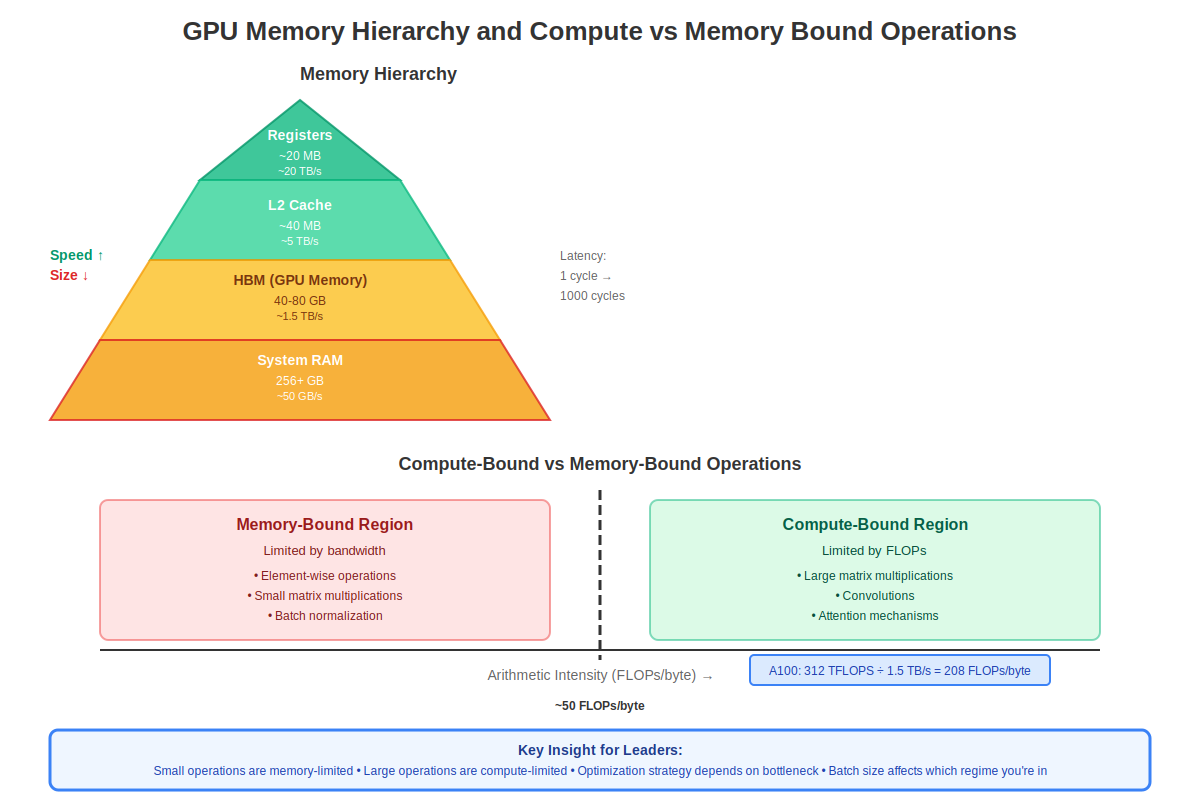
\includegraphics[width=0.9\textwidth]{chapters/diagrams/chapter01_memory_hierarchy_8aa29564.pdf}
\caption{GPU memory hierarchy and compute-memory trade-offs. Understanding when operations are memory-bound versus compute-bound informs optimization strategies.}
\label{fig:memory_hierarchy}
\end{figure}


\section{Model Compression and Optimization}

\subsection{Compression Techniques}

Production deployments frequently employ compression techniques to reduce resource requirements while maintaining acceptable performance. Three primary approaches have demonstrated effectiveness:

\textbf{Knowledge Distillation}: Training a smaller model to replicate a larger model's behavior. Typical results achieve 50\% parameter reduction with 2-3\% accuracy degradation. This approach is particularly effective for deployment scenarios where inference cost dominates total cost of ownership.

\textbf{Quantization}: Reducing numerical precision from 32-bit to 8-bit or 16-bit representations. This technique provides 2-4× memory reduction with minimal accuracy impact (<1\% typically). Modern hardware includes specialized support for lower-precision arithmetic, enabling both memory and computational benefits.

\textbf{Pruning}: Removing parameters with minimal impact on model performance. Structured pruning can achieve 30-50\% parameter reduction while maintaining performance within acceptable bounds. This technique requires careful validation to ensure pruned models maintain robustness across diverse inputs.

\subsection{Economic Implications}

For high-volume production systems, compression techniques translate directly to infrastructure cost reduction. A 50\% model size reduction through distillation enables:
\begin{itemize}
    \item Reduced memory requirements, potentially enabling deployment on less expensive hardware
    \item Decreased inference latency, improving user experience and enabling higher throughput
    \item Lower operational costs through reduced computational requirements
\end{itemize}

These benefits compound at scale. For systems serving millions of requests daily, compression-driven efficiency improvements can reduce annual infrastructure costs by hundreds of thousands of dollars.

\section{Evaluation Framework}

\subsection{Architectural Assessment Criteria}

When evaluating model architecture proposals, consider:

\textbf{Dimensional Specifications}:
\begin{itemize}
    \item What dimensional parameters are proposed, and what is the technical justification?
    \item How do proposed dimensions compare to established baselines for similar applications?
    \item What is the expected accuracy-cost trade-off relative to alternative dimensions?
\end{itemize}

\textbf{Parameter Allocation}:
\begin{itemize}
    \item What is the total parameter count, and how does it compare to comparable models?
    \item Where are parameters concentrated, and does this allocation align with model objectives?
    \item Have smaller models been evaluated to establish the accuracy-parameter relationship?
\end{itemize}

\textbf{Resource Requirements}:
\begin{itemize}
    \item What are the memory requirements for training versus inference?
    \item What batch sizes are feasible given available hardware?
    \item Have compression techniques been considered for production deployment?
\end{itemize}

\subsection{Common Evaluation Pitfalls}

\textbf{Overemphasis on Parameter Count}: Parameter count alone provides incomplete information. A well-designed 50M parameter model may outperform a poorly-designed 200M parameter model. Architecture quality and training methodology matter as much as raw parameter count.

\textbf{Conflating Training and Inference Costs}: Training costs are one-time investments; inference costs are ongoing operational expenses. For high-volume applications, inference efficiency often matters more than training efficiency.

\textbf{Insufficient Baseline Comparison}: Proposals should include comparison to established baselines. Claims of superior performance require validation against recognized benchmarks, not just internal metrics.

\textbf{Neglecting Compression Opportunities}: Production deployment should consider compression from the outset, not as a post-deployment optimization. Early integration of compression techniques into the development process yields better results.

\begin{tcolorbox}[colback=red!5!white,colframe=red!75!black,title=\textbf{CAUTIONARY TALE: The Model That Didn't Fit in Memory}]

\textbf{What Happened:}

A fintech startup decided to train a custom BERT-large variant (340M parameters) for financial document analysis. Their team had access to 4× V100 GPUs (16GB each) and estimated training would take 2 weeks.

\textbf{Week 1:} Training failed immediately with out-of-memory errors. Investigation revealed they calculated only parameter memory (1.3GB) but ignored the 14× rule. Actual requirement: 18GB per GPU at their planned batch size of 64.

\textbf{Attempted Fix:} Reduced batch size to 8 (fits in 16GB). Training started but was 8× slower than estimated—would take 16 weeks instead of 2. GPU utilization dropped to 15\% (memory-bound, not compute-bound).

\textbf{Outcome:}

Project timeline blown. Emergency pivot: Switched to BERT-base (110M parameters, 6GB training memory), batch size 32, completed in 3 weeks. Final model achieved 94\% of BERT-large's accuracy at 1/4 the training cost and 1/3 the inference cost.

\textbf{Lesson:} Always apply the 14× memory rule when planning training infrastructure. Parameter count alone is misleading. Batch size dramatically affects both memory requirements and training efficiency. When memory-constrained, smaller models with proper batch sizes often outperform larger models with tiny batches.

\textbf{Red Flags They Missed:}
\begin{itemize}
    \item No memory calculation beyond parameter storage
    \item No consideration of optimizer state (2× parameters)
    \item No activation memory estimate (4-6× parameters)
    \item No GPU utilization analysis before committing
\end{itemize}

\end{tcolorbox}

\section{Where You'll See This in Practice}

The architectural concepts in this chapter underpin multiple domain applications you'll encounter in Part IV:

\subsection{Legal Document Analysis (Chapter 13)}

Contract analysis systems processing 50-page documents face the same quadratic attention scaling discussed in Section 1.1.3. When your legal team proposes analyzing 100-page merger agreements, 50 pages (≈12K tokens) versus 100 pages (≈24K tokens) equals 4× attention cost. The parameter distribution patterns (Section 1.2.1) determine which compression techniques work. Inference optimization (Section 1.2.3) becomes critical when processing thousands of contracts.

\textbf{Decision point}: Should you chunk long documents (cheaper) or use long-context models (higher quality)? Section 1.1.4's memory-compute trade-offs provide the framework.

\subsection{Financial Time Series (Chapter 14)}

TabTransformer architecture for credit risk (Chapter 14.2) follows the same parameter scaling principles. Embedding dimensions scale cubically just like BERT (Section 1.1.2). FFN-dominated parameter counts (Section 1.2.1) appear in financial models too. Training memory overhead (13× rule from Section 1.2.2) applies universally.

\textbf{Decision point}: When vendors propose "custom financial transformers," you can now calculate whether the parameter count matches their claimed model size.

\subsection{Code Generation (Chapter 11)}

GitHub Copilot-style systems face context window trade-offs: How much code history to include? (Section 1.1.3). Parameter efficiency: Specialized code models versus general LLMs (Section 1.2.1). Inference cost at scale: Millions of autocomplete requests daily (Section 1.2.3).

\textbf{Decision point}: Self-host a smaller model (lower per-request cost) or use API (higher cost, better quality)? The memory requirements from Section 1.2.2 determine what hardware you'll need.

\subsection{Healthcare NLP (Chapter 12)}

Clinical text processing systems must balance accuracy requirements with inference costs (Section 1.2.3), deploy on-premise due to HIPAA (Section 1.2.2 memory requirements become critical), and compress models for edge deployment in hospitals (Section 1.4).

\textbf{Decision point}: Can you quantize to INT8 (4× smaller) without violating accuracy requirements? Section 1.4's compression techniques provide the evaluation framework.

\subsection{Enterprise Search (Chapter 10)}

Semantic search with RAG systems involves embedding models for 10M documents (Section 1.2.1 parameter efficiency), real-time query latency requirements (Section 1.2.3 inference optimization), and cost at scale: 100K queries/day (Section 1.3 scaling analysis).

\textbf{Decision point}: Use general-purpose BERT or fine-tune domain-specific embeddings? Section 1.4's compression economics help calculate ROI.

\subsection{Key Takeaway}

The architectural principles in this chapter aren't abstract theory—they're the foundation for evaluating every AI proposal you'll face. When your team suggests "upgrading to a larger model" or "extending context windows," you now have the frameworks to calculate the actual cost impact (cubic versus quadratic versus linear scaling), identify optimization opportunities (where are parameters concentrated?), and make informed trade-offs (quality versus cost versus latency). Bookmark this chapter—you'll reference it constantly when evaluating proposals in Part IV.

\section{Key Insights}

\textbf{Non-linear Scaling}: Computational costs scale cubically with model dimension, while memory scales quadratically. Small dimensional increases produce large resource requirement increases.

\textbf{Parameter Distribution}: In transformer architectures, feed-forward networks typically contain 50-60\% of parameters despite conceptual simplicity. This concentration represents an optimization opportunity.

\textbf{Training-Inference Disparity}: Training memory requirements exceed inference requirements by 6-10×, primarily due to activation storage. Infrastructure planning should account for these distinct profiles.

\textbf{Diminishing Returns}: Model scaling exhibits diminishing returns. BERT-large requires 4× more resources than BERT-base for 2-3\% accuracy improvement, illustrating the cost-benefit trade-off at larger scales.

\textbf{Compression Viability}: Most production models can be compressed 2-4× with minimal accuracy impact. This capability should inform deployment strategies and infrastructure planning.

The next chapter examines training dynamics—how these models are optimized, what drives training costs, and how to evaluate training efficiency proposals.

